\documentclass[conference]{IEEEtran}
\usepackage[T1]{fontenc}
\usepackage{amsmath,amssymb}
\usepackage{graphicx}
\usepackage{booktabs}
\usepackage{listings}
\lstset{language=Matlab,basicstyle=\ttfamily\scriptsize,breaklines=true,
columns=fullflexible,keepspaces=true,numbers=left,numberstyle=\tiny,
numbersep=4pt,frame=single,tabsize=4,showstringspaces=false}
\usepackage[hidelinks]{hyperref}
\graphicspath{{images/}}
\newcommand{\diag}{\operatorname{diag}}
\newcommand{\rank}{\operatorname{rank}}
\newcommand{\eig}{\operatorname{eig}}
\newcommand{\dd}{\mathrm{d}}

\title{MA6217 Project Report}
% Add the student names and matriculation numbers here before submission.
\author{\IEEEauthorblockN{Group 7}
\IEEEauthorblockA{Liu Bingnan, Vilayanur Adithya Haridas, Xu Siyu, Yang Jiaxin, Zhang Mengliu}}

\begin{document}
\maketitle

\section{Introduction}

The rotary inverted pendulum is unstable at its upright equilibrium, and keeping it balanced while repositioning the rotary arm requires feedback control. The arm and pendulum angles are measured directly, while their angular velocities are estimated using a Kalman observer. An LQR controller is first designed to stabilize the pendulum, then combined with a reference feedforward gain to track commanded arm angles with zero nominal steady-state error. The model, observer, and controllers are developed in state-space form and evaluated through linear and nonlinear simulations.

\begin{figure}[t]
\centering
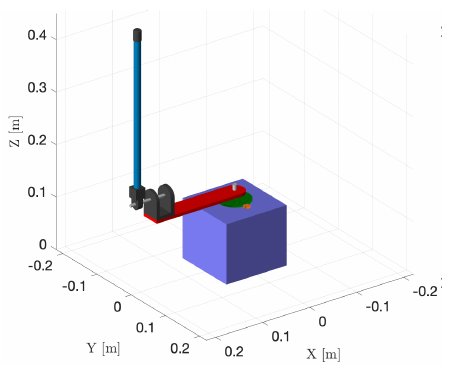
\includegraphics[width=0.65\columnwidth]{rotary_pendulum.png}
\caption{Rotary inverted pendulum system.}
\label{fig:plant}
\end{figure}

\section{State Space Model}

\subsection{State and Input Definitions}

The rotary arm angle is denoted by $\theta$, and $\alpha$ measures the pendulum angle from its upright position. Both angles are measured, while their angular velocities complete the four-dimensional state vector. With motor voltage $u$ as the control input, the state and output vectors are

\begin{equation}
x=\begin{bmatrix}\theta&\alpha&\dot\theta&\dot\alpha\end{bmatrix}^{T},
\qquad y=\begin{bmatrix}\theta&\alpha\end{bmatrix}^{T}.
\label{eq:state}
\end{equation}

Near the upright equilibrium, the dynamics can be written in linear state-space form as

\begin{equation}
\dot x=Ax+Bu,\qquad y=Cx+Du.
\label{eq:model}
\end{equation}

\subsection{Derivation of the System Matrices}

Table \ref{tab:parameters} lists the physical and motor parameters. Taking the pendulum's center of mass to be at $l_p=L_p/2$, the inertias and mechanical coupling terms are

\begin{equation}
\begin{aligned}
J_p&=\frac{m_pL_p^2}{12}, &J&=\frac{m_rr_a^2}{3}+J_{\mathrm{rot}},\\
M_a&=J+m_pr_a^2, &H_p&=J_p+m_pl_p^2,\\
c&=m_pl_pr_a, &h_g&=m_pl_pg.
\end{aligned}
\label{eq:coefficients}
\end{equation}

\begin{table}[t]
\caption{Model Parameters}
\label{tab:parameters}
\centering\small
\begin{tabular}{@{}lll@{}}
\toprule
Quantity & Symbol & Value\\
\midrule
Pendulum mass & $m_p$ & $0.127$ kg\\
Pendulum length & $L_p$ & $0.33655$ m\\
Arm mass & $m_r$ & $0.257$ kg\\
Arm length & $r_a$ & $0.2159$ m\\
Reflected drive inertia & $J_{\mathrm{rot}}$ & $0.002087$ kg\,m$^2$\\
Gear ratio & $G$ & $70$\\
Armature resistance & $R_a$ & $2.6\,\Omega$\\
Torque constant & $k_t$ & $0.00768$ N\,m/A\\
Back-EMF constant & $k_b$ & $0.00768$ V\,s/rad\\
Motor efficiency & $\eta_m$ & $0.69$\\
Gear efficiency & $\eta_g$ & $0.90$\\
Arm and pendulum damping & $B_r,B_p$ & $0.0024$ N\,m\,s/rad\\
Gravitational acceleration & $g$ & $9.81$ m/s$^2$\\
\bottomrule
\end{tabular}
\end{table}

The effective motor torque coefficient and arm damping coefficient are

\begin{equation}
k_v=\frac{\eta_gG\eta_mk_t}{R_a},\qquad
d_v=B_r+k_vGk_b.
\label{eq:motor}
\end{equation}

Linearizing about the upright equilibrium $\alpha=0$ with $\sin\alpha\approx\alpha$ and $\cos\alpha\approx1$ gives the coupled mechanical equations

\begin{equation}
\begin{bmatrix}M_a&-c\\-c&H_p\end{bmatrix}
\begin{bmatrix}\ddot\theta\\\ddot\alpha\end{bmatrix}
=\begin{bmatrix}k_vu-d_v\dot\theta\\h_g\alpha-B_p\dot\alpha\end{bmatrix}.
\label{eq:mechanics}
\end{equation}

Inverting the mass matrix with $\Delta=M_aH_p-c^2$ and arranging the angular accelerations in state-space form gives

\begin{equation}
A=\begin{bmatrix}
0&0&1&0\\
0&0&0&1\\
0&ch_g/\Delta&-H_pd_v/\Delta&-cB_p/\Delta\\
0&M_ah_g/\Delta&-cd_v/\Delta&-M_aB_p/\Delta
\end{bmatrix},
\label{eq:Asymbolic}
\end{equation}

\begin{equation}
B=\begin{bmatrix}0&0&H_pk_v/\Delta&ck_v/\Delta\end{bmatrix}^{T}.
\label{eq:Bsymbolic}
\end{equation}

Using the parameter values in Table \ref{tab:parameters}, the numerical system matrices are

\begin{equation}
\setlength{\arraycolsep}{3.5pt}
A\approx\begin{bmatrix}
0&0&1&0\\
0&0&0&1\\
0&26.6844&-9.4482&-0.3055\\
0&69.4005&-9.0917&-0.7945
\end{bmatrix},\quad
B\approx\begin{bmatrix}0\\0\\16.9843\\16.3434\end{bmatrix}.
\label{eq:ABnumerical}
\end{equation}

\begin{equation}
C=\begin{bmatrix}1&0&0&0\\0&1&0&0\end{bmatrix},\qquad D=0_{2\times1}.
\label{eq:CD}
\end{equation}

\subsection{Controllability and Observability}

Controllability and observability are checked using

\begin{equation}
\mathcal C=\begin{bmatrix}B&AB&A^2B&A^3B\end{bmatrix},\quad
\mathcal O=\begin{bmatrix}C\\CA\\CA^2\\CA^3\end{bmatrix}.
\label{eq:ranks}
\end{equation}

Both matrices have rank four. Thus, the motor input can control all four states, and the measured angles provide enough information to reconstruct the full state. The open-loop poles are

\begin{equation}
\eig(A)\approx\{0,\ 7.0915,\ -12.7738,\ -4.5604\}\ \mathrm{s}^{-1}.
\label{eq:openpoles}
\end{equation}

The positive real pole confirms that the upright equilibrium is unstable without feedback.

\section{Kalman State Estimation}

\subsection{Observer Design}

The feedback controller requires both angular velocities, which are not measured directly. A Kalman observer estimates them from the two measured angles and the applied motor voltage. Process and measurement noise are included in the observer design model:

\begin{equation}
\dot x=Ax+Bu+G_nw,\qquad y=Cx+v.
\label{eq:noise_model}
\end{equation}

Here $w$ and $v$ are uncorrelated, zero-mean white process and measurement noises with intensity matrices $Q_n$ and $R_n$. The observer is designed with

\begin{equation}
G_n=\begin{bmatrix}0&0\\0&0\\1&0\\0&1\end{bmatrix},\qquad
Q_n=10I_2,\qquad R_n=I_2.
\label{eq:noisew}
\end{equation}

Writing $\hat x$ for the estimated state, the innovation $\nu=y-C\hat x$ measures the difference between the observed angles and their model-based predictions. The observer uses this difference to correct the state estimate:

\begin{equation}
\dot{\hat x}=A\hat x+Bu +L\nu.
\label{eq:observer}
\end{equation}

For the estimation error $\tilde x=x-\hat x$, the error dynamics are

\begin{equation}
\dot{\tilde x}=(A-LC)\tilde x+G_nw-Lv.
\label{eq:esterror}
\end{equation}

The estimation-error covariance is $P=\mathbb E[\tilde x\tilde x^T]$. With $W=G_nQ_nG_n^T$, its dynamics satisfy

\begin{equation}
\dot P=(A-LC)P+P(A-LC)^T+W+LR_nL^T.
\label{eq:covariance}
\end{equation}

Rearranging this expression by completing the square, where $L_\star=PC^TR_n^{-1}$, gives

\begin{equation}
\begin{split}
\dot P={}&AP+PA^T+W-PC^TR_n^{-1}CP\\
&+(L-L_\star)R_n(L-L_\star)^T.
\end{split}
\label{eq:covsquare}
\end{equation}

The final term is minimized by $L=L_\star$. Setting $\dot P=0$ then yields the steady-state estimator Riccati equation

\begin{equation}
AP_e+P_eA^T-P_eC^TR_n^{-1}CP_e+W=0,
\label{eq:estcare}
\end{equation}

The stabilizing solution $P_e$ determines the Kalman gain

\begin{equation}
L=P_eC^TR_n^{-1}\approx
\begin{bmatrix}
1.0331&2.6290\\2.6290&13.6995\\
3.9893&20.2496\\18.4818&97.2939
\end{bmatrix}.
\label{eq:L}
\end{equation}

The resulting error-dynamics poles are

\begin{equation}
\begin{split}
\eig(A-LC)\approx\{&-12.7726,-7.0700,\\
&-4.5614,-0.5714\}\ \mathrm{s}^{-1}.
\end{split}
\label{eq:obspoles}
\end{equation}

All four poles lie in the left half-plane, so the estimation error converges in the absence of noise. In the simulation, the observer receives $[u,\theta,\alpha]^T$ and is implemented with the state-space matrices

\begin{equation}
\begin{aligned}
A_{\mathrm{obs}}&=A-LC,& B_{\mathrm{obs}}&=\begin{bmatrix}B&L\end{bmatrix},\\
C_{\mathrm{obs}}&=I_4,& D_{\mathrm{obs}}&=0_{4\times3}.
\end{aligned}
\label{eq:obsimplementation}
\end{equation}

\subsection{Noise Weight Comparison}

The process-noise and measurement-noise weights determine how strongly the observer responds to differences between predicted and measured angles. Larger $Q_n$ relative to $R_n$ generally increases the influence of the measurements, while larger $R_n$ reduces it.

To examine the effect of these weights, $R_n=I_2$ is fixed and $Q_n=qI_2$ is varied across 40 logarithmically spaced values from $0.01$ to $1000$. The initial error is $\tilde x(0)=[0.1,-0.05,0.3,-0.2]^T$. Each noise-free error response is simulated for $60$ s with a sampling interval of $0.05$ s.

The comparison focuses on the pendulum-speed estimation error, $e_4=\dot\alpha-\widehat{\dot\alpha}$. Its settling time $T_s$ is the first sampled time after which $|e_4|$ stays below $0.004$ rad/s for the remainder of the test, corresponding to $2\%$ of the initial error magnitude. The peak $|e_4|$ and the slowest error-dynamics pole, $\sigma=\max_i\operatorname{Re}\lambda_i(A-LC)$, are also recorded.

\begin{figure}[t]
\centering
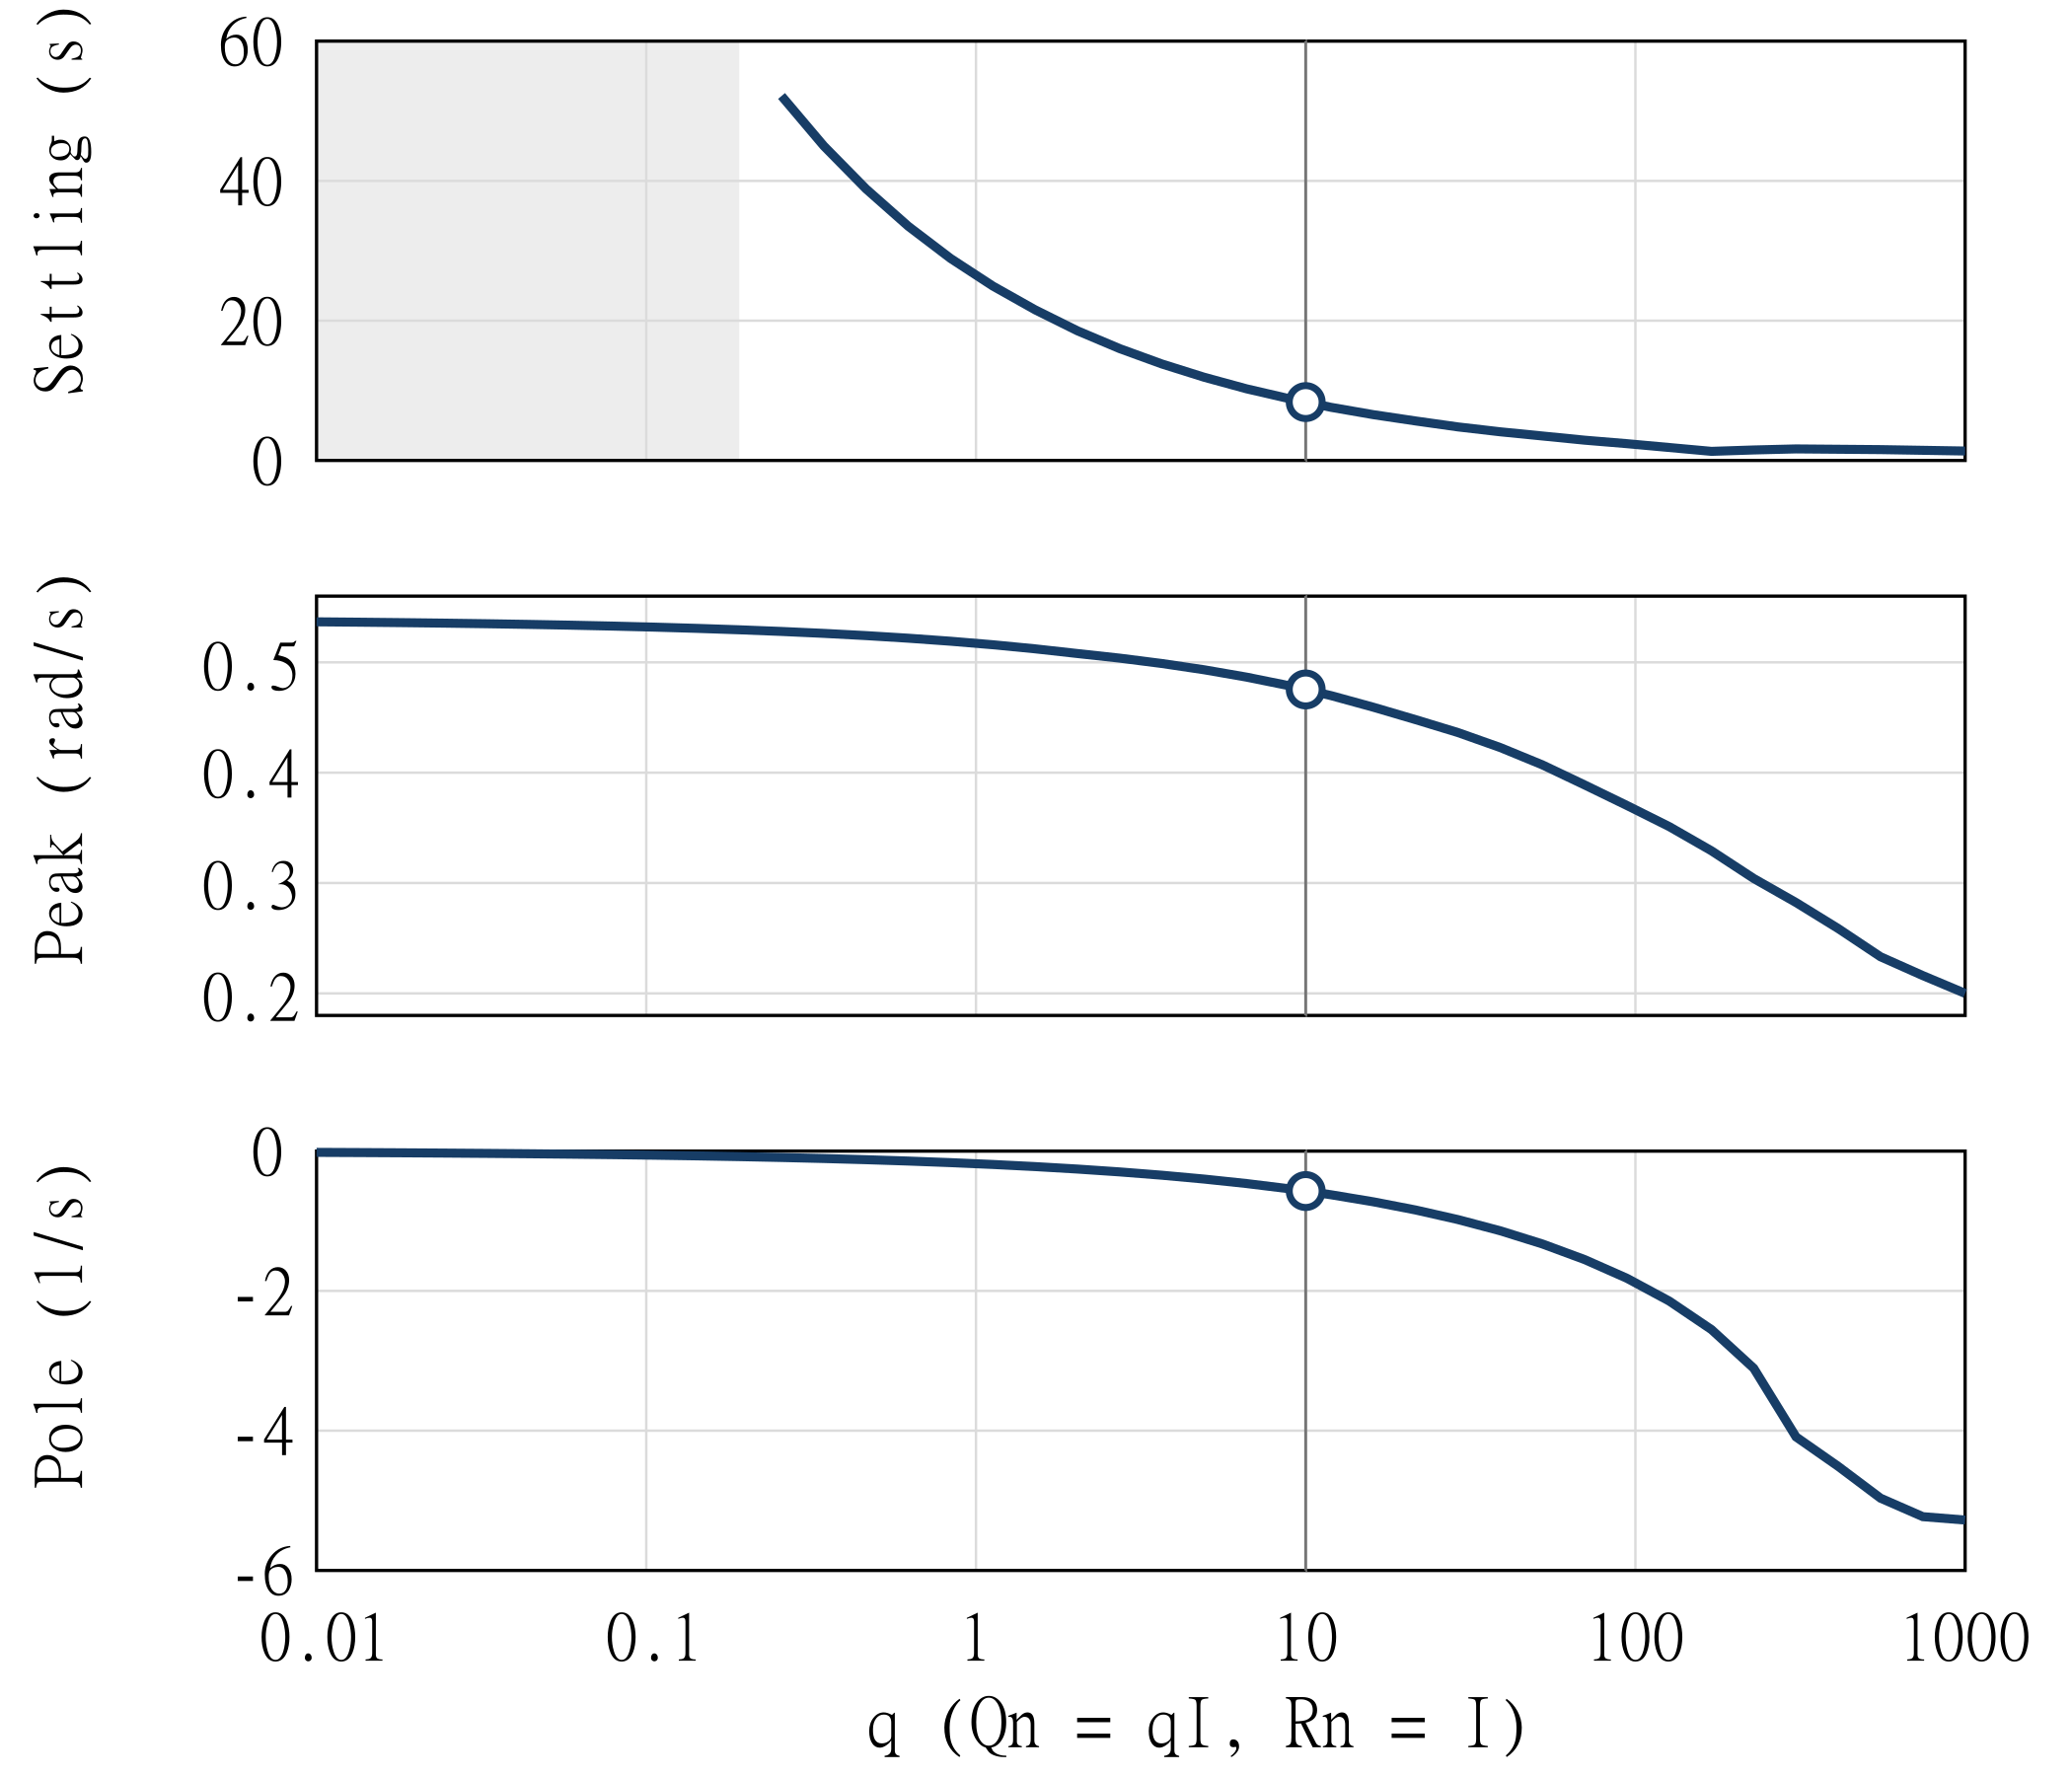
\includegraphics[width=\columnwidth]{observer_sensitivity.png}
\caption{LQE weight comparison. Shading marks cases with $T_s>60$ s; circles mark the nominal setting $q=10$.}
\label{fig:kalman_sweep}
\end{figure}

\begin{table}[t]
\caption{Kalman Weight Comparison}
\label{tab:kalman_sweep}
\centering\small
\begin{tabular}{@{}rrrr@{}}
\toprule
$q$ & $T_s$ (s) & Peak $|e_4|$ (rad/s) & $\sigma$ (s$^{-1}$)\\
\midrule
0.01 & $>60$ & 0.5367 & $-0.0180$\\
10 & 8.35 & 0.4754 & $-0.5714$\\
170.13 & 1.30 & 0.3292 & $-2.5540$\\
1000 & 1.35 & 0.2000 & $-5.2790$\\
\bottomrule
\end{tabular}
\end{table}

Figure \ref{fig:kalman_sweep} and Table \ref{tab:kalman_sweep} show a clear reduction in estimation error as $q$ increases. At $q=0.01$, the settling time exceeds $60$ s and the peak error is $0.5367$ rad/s. With $q=10$, the settling time falls to $8.35$ s; at $q=1000$, it is $1.35$ s and the peak error falls to $0.2000$ rad/s. Although the slowest pole continues moving left, settling time increases slightly from $1.30$ s at $q=170.13$ to $1.35$ s at $q=1000$, reflecting the complete transient response relative to the settling threshold. The balancing and feedforward tracking simulations both retain $Q_n=10I_2$ and $R_n=I_2$.

\subsection{Velocity Estimation Results}

The observer is then tested during an $8$ s nonlinear balancing simulation, starting from $\alpha(0)=5^\circ$ and $\hat x(0)=0$. As shown in Fig. \ref{fig:recovery}, the estimated angular velocities approach their true values as the pendulum recovers. During the final second, the maximum absolute errors are $3.9799\times10^{-5}$ rad/s for the arm velocity and $1.7912\times10^{-4}$ rad/s for the pendulum velocity.

\begin{figure}[t]
\centering
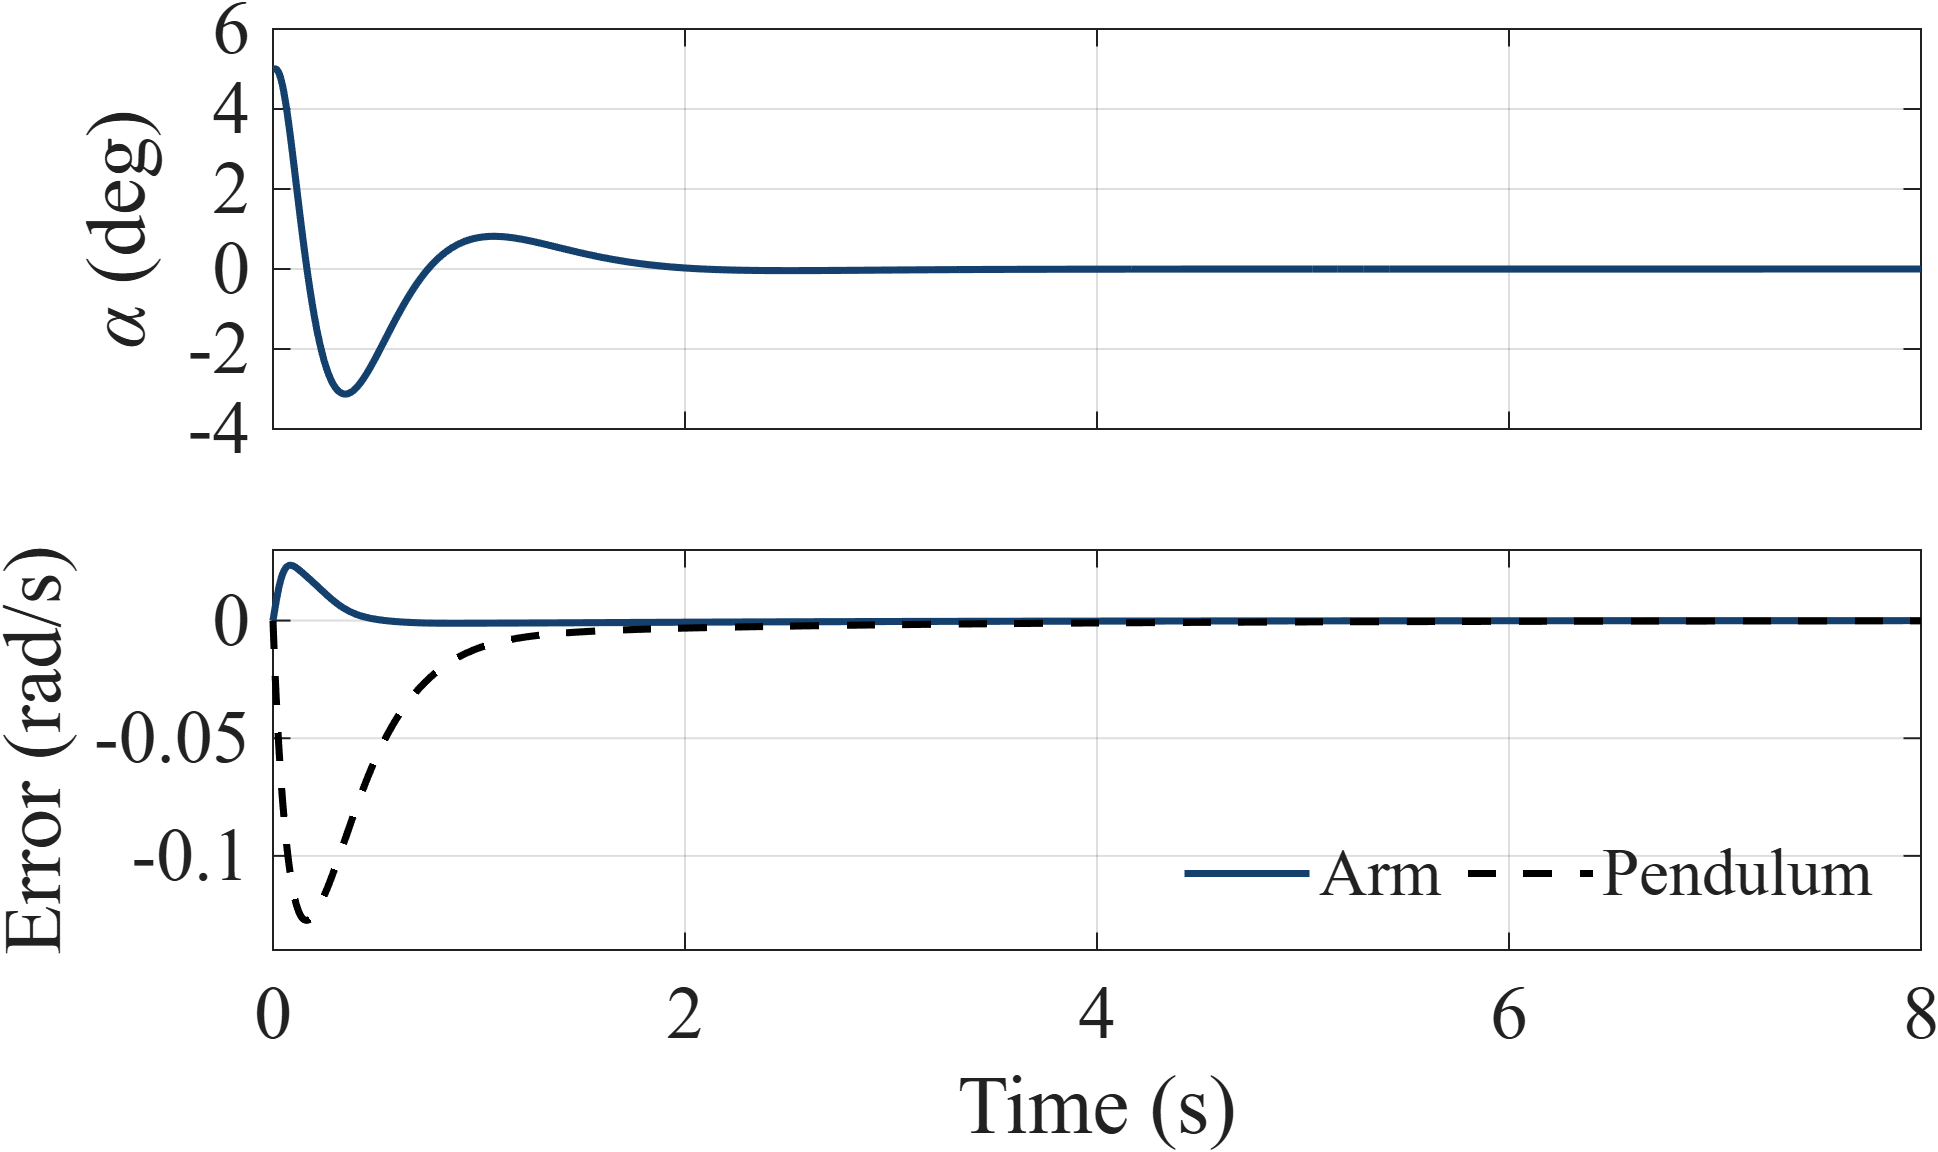
\includegraphics[width=\columnwidth]{step2_recovery.png}
\caption{Nonlinear balancing response and velocity estimation errors. Errors are true values minus estimates.}
\label{fig:recovery}
\end{figure}

\section{LQR Stabilization}

\subsection{Optimal State Feedback}

Once the states can be estimated, feedback is used to return the pendulum to its upright equilibrium. The LQR controller is obtained by minimizing the infinite-horizon quadratic cost

\begin{equation}
J_c=\int_0^\infty(x^TQ_cx+R_cu^2)\dd t,
\qquad Q_c\succ0,\quad R_c>0.
\label{eq:lqrcost}
\end{equation}

The matrix $Q_c$ penalizes state deviations, while $R_c$ penalizes the motor voltage. Assuming a quadratic optimal value function $V(x)=x^TP_cx$, the Hamilton--Jacobi--Bellman equation becomes

\begin{equation}
0=\min_u\{x^TQ_cx+R_cu^2+2x^TP_c(Ax+Bu)\}.
\label{eq:hjb}
\end{equation}

Minimizing with respect to $u$ gives $2R_cu+2B^TP_cx=0$, leading to the feedback law

\begin{equation}
u^\star=-Kx,\qquad K=R_c^{-1}B^TP_c.
\label{eq:gainformula}
\end{equation}

Substituting the feedback law into the Hamilton--Jacobi--Bellman equation gives the continuous-time algebraic Riccati equation

\begin{equation}
A^TP_c+P_cA-P_cBR_c^{-1}B^TP_c+Q_c=0.
\label{eq:controlcare}
\end{equation}

For the stabilizing solution $P_c$, the derivative of $V=x^TP_cx$ along the closed-loop trajectories is

\begin{equation}
\dot V=-x^T(Q_c+K^TR_cK)x<0\qquad(x\ne0).
\label{eq:lyapunov}
\end{equation}

The negative derivative establishes asymptotic stability of the state-feedback system.

\subsection{Weight Comparison and Selected Controller}

The controller weights determine how aggressively the pendulum is balanced and how much motor voltage is used. Four choices are compared with $Q_c=\diag(10,q_\alpha,1,10)$ using the linear model. Each simulation starts from $x(0)=[0,5\pi/180,0,0]^T$ and runs for $5$ s. Figure \ref{fig:lqr_weights} shows the angle and voltage responses, and Table \ref{tab:lqr} reports their peak values.

\begin{table}[t]
\caption{LQR Weight Comparison}
\label{tab:lqr}
\centering\small
\begin{tabular}{@{}ccccc@{}}
\toprule
Case & $q_\alpha$ & $R_c$ & Peak $|\theta|$ ($^\circ$) & Peak $|u|$ (V)\\
\midrule
1 & 100 & 1 & 12.57 & 3.76\\
2 & 300 & 1 & 12.14 & 4.06\\
3 & 100 & 0.1 & 11.84 & 10.26\\
4 & 100 & 10 & 14.09 & 1.91\\
\bottomrule
\end{tabular}
\end{table}

Increasing the pendulum-angle weight $q_\alpha$ from $100$ to $300$ reduces the peak arm rotation from $12.57^\circ$ to $12.14^\circ$, while the peak voltage rises by only $0.30$ V, from $3.76$ to $4.06$ V. Case 3 produces a slightly smaller peak arm angle of $11.84^\circ$, but requires $10.26$ V. In contrast, Case 4 limits the peak voltage to $1.91$ V while allowing the arm to rotate by $14.09^\circ$. Case 2 is therefore used for the remaining simulations: compared with the baseline, it reduces arm motion with a modest increase in voltage, without the much larger control demand of Case 3.

\begin{figure}[t]
\centering
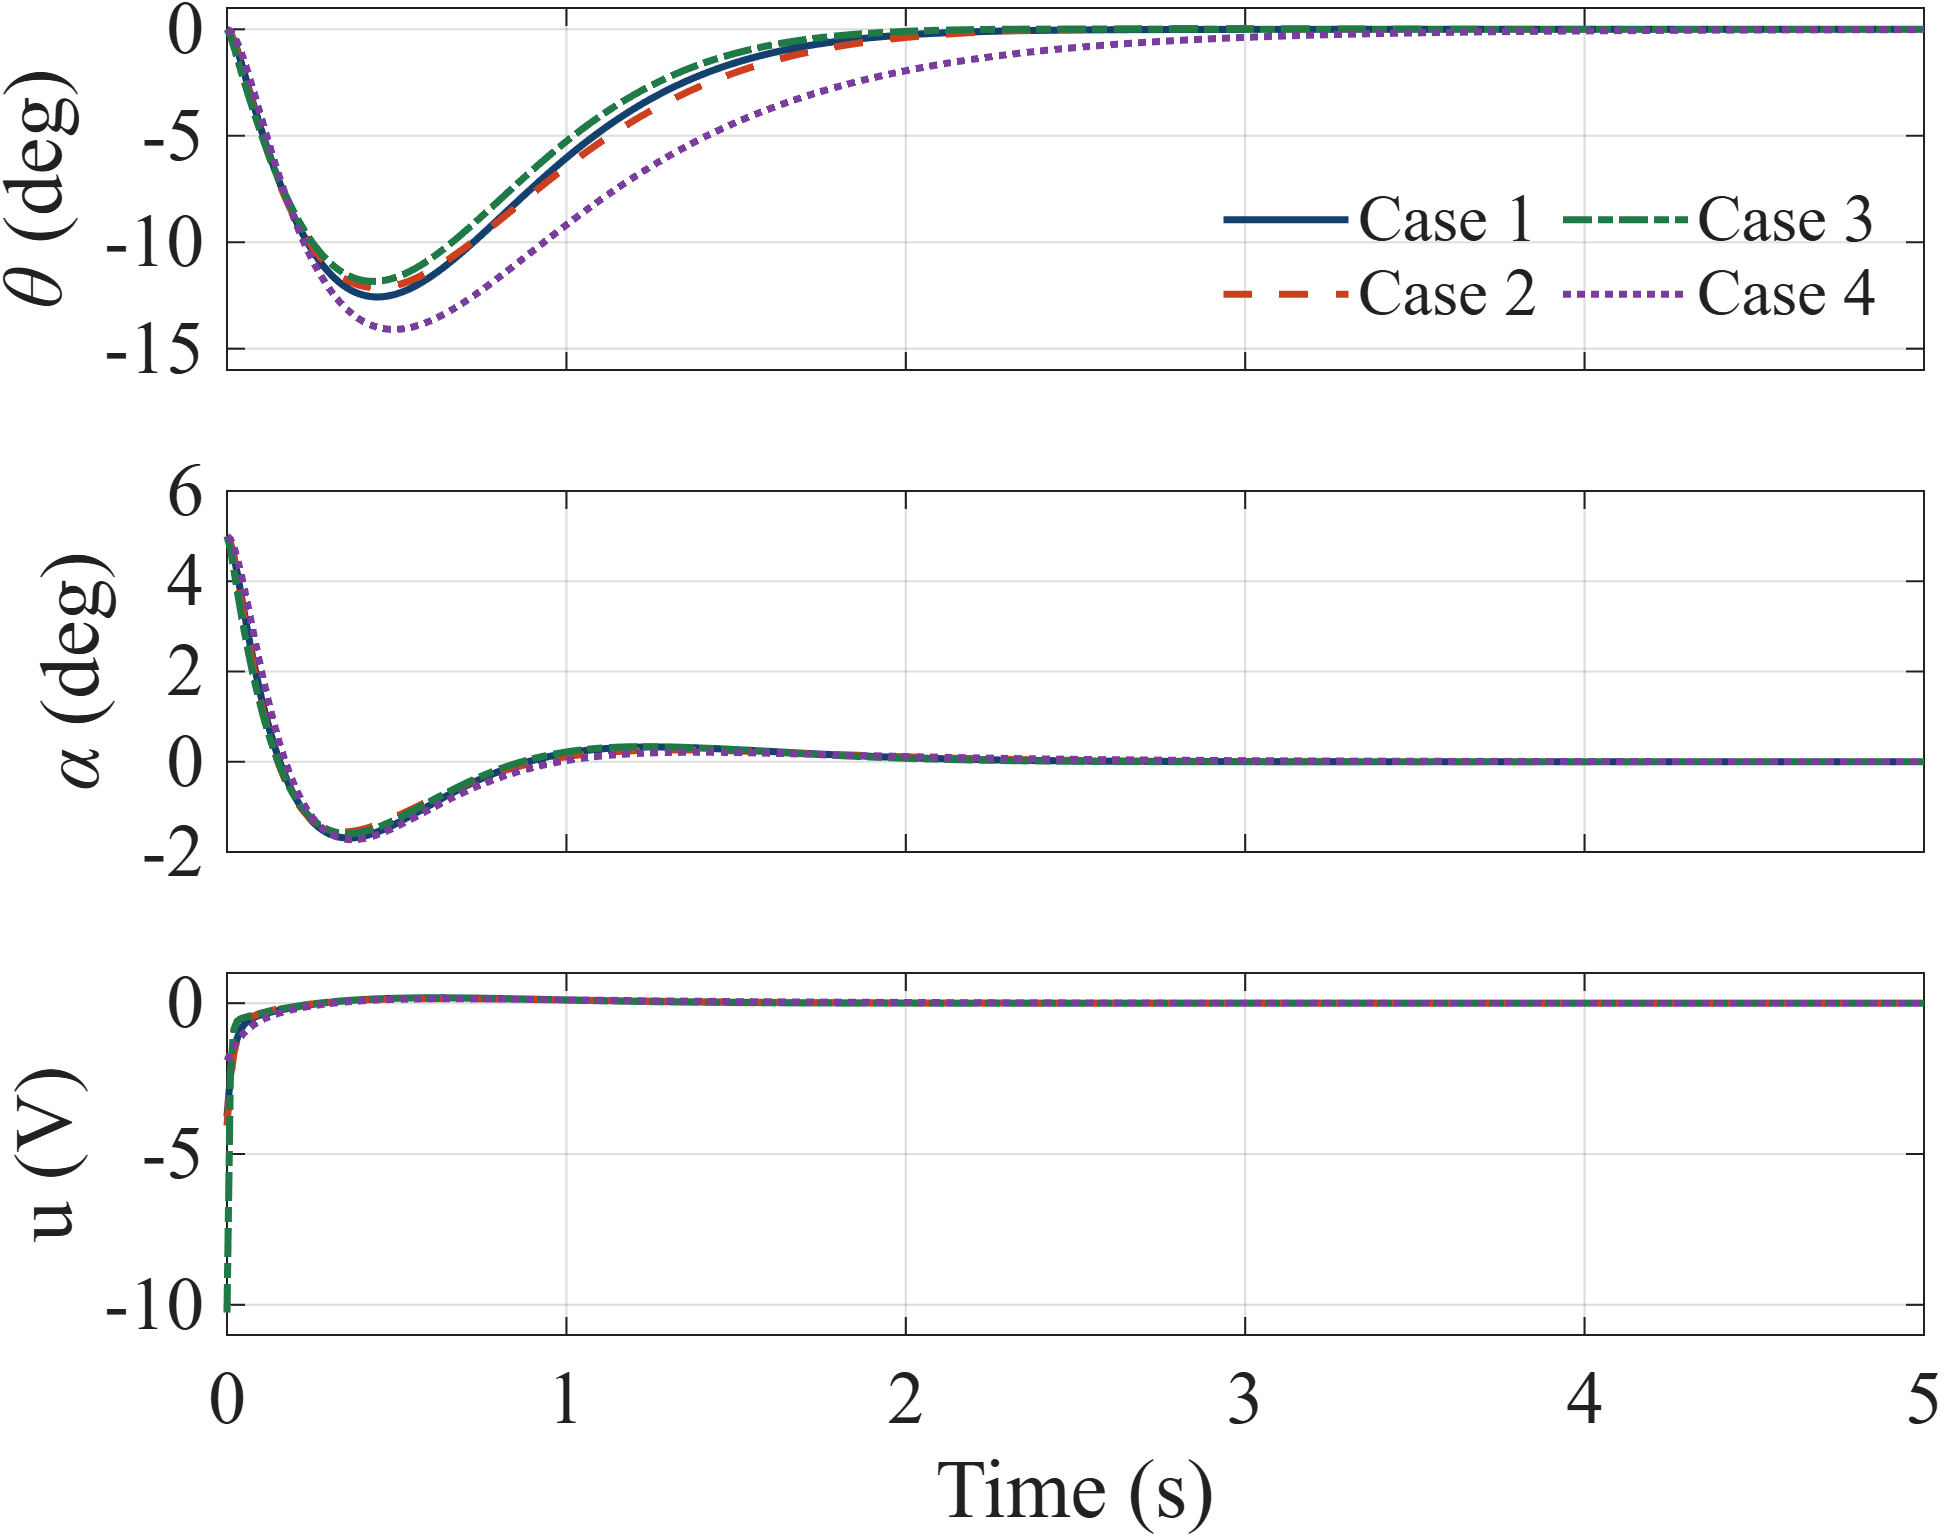
\includegraphics[width=\columnwidth]{lqr_weight_comparison.png}
\caption{LQR responses for the four weight choices in Table \ref{tab:lqr}, with an initial pendulum tilt of $5^\circ$. Case 2 is selected.}
\label{fig:lqr_weights}
\end{figure}

For Case 2, the feedback gain and closed-loop poles are

\begin{equation}
K=\begin{bmatrix}-3.1623&46.5279&-3.2386&6.8080\end{bmatrix},
\label{eq:K}
\end{equation}

\begin{equation}
\begin{split}
\eig(A-BK)\approx\{&-56.1744,-5.4649,\\
&-2.4325\pm j1.3163\}\ \mathrm{s}^{-1}.
\end{split}
\label{eq:regpoles}
\end{equation}

In the observer-based implementation, $\hat x$ replaces the unavailable full state, giving $u=-K\hat x$. With the combined coordinates $[x^T,\tilde x^T]^T$, the dynamics can be written as

\begin{equation}
\begin{bmatrix}\dot x\\\dot{\tilde x}\end{bmatrix}
=\begin{bmatrix}A-BK&BK\\0&A-LC\end{bmatrix}
\begin{bmatrix}x\\\tilde x\end{bmatrix}.
\label{eq:separation}
\end{equation}

Because this matrix is block triangular, its eigenvalues are the poles of $A-BK$ and $A-LC$. Both sets lie in the left half-plane, so the observer and regulator form a stable LQG closed loop. The same structure explains why their gains can be designed separately.

\subsection{Balancing Results}

The nonlinear balancing simulation begins with a $5^\circ$ pendulum tilt, all other physical states set to zero, and $\hat x(0)=0$. Figure \ref{fig:recovery} shows the pendulum returning upright as the arm moves to recover balance. The maximum arm angle is $15.0733^\circ$, and the peak motor voltage is $1.3932$ V. During the final second, from $7$ to $8$ s, the maximum absolute arm and pendulum angles decrease to $0.0746441^\circ$ and $0.000536751^\circ$, respectively.

The voltage transient differs from the earlier linear full-state comparison because the controller initially acts on an estimated state rather than the true state. Full-state feedback gives $u(0)\approx-4.0603$ V, whereas $\hat x(0)=0$ makes the initial observer-based command $u(0)=0$.

\section{Reference Tracking with Feedforward}

\subsection{Reference Gain Design}

The arm reference $r$ is introduced through a static feedforward gain while retaining the LQR gain $K$ selected in Step 2. The control law is

\begin{equation}
u=-K\hat x+N_{\mathrm{bar}}r.
\label{eq:feedforward}
\end{equation}

Thus, the tracking controller uses the same state weights $Q_c=\diag(10,300,1,10)$ and input weight $R_c=1$. The Kalman observer also retains $Q_n=10I_2$ and $R_n=I_2$.

For a constant reference, write the desired steady state and input as $x_{\mathrm{ss}}=N_xr$ and $u_{\mathrm{ss}}=N_ur$. They satisfy

\begin{equation}
AN_x+BN_u=0,\qquad C_\theta N_x=1,
\label{eq:steadyconditions}
\end{equation}

where $C_\theta=[1,0,0,0]$ selects the arm angle. The two conditions can be solved together:

\begin{equation}
\begin{bmatrix}A&B\\C_\theta&0\end{bmatrix}
\begin{bmatrix}N_x\\N_u\end{bmatrix}
=\begin{bmatrix}0_{4\times1}\\1\end{bmatrix}.
\label{eq:steadysolve}
\end{equation}

At steady state, the control law must supply $N_ur=-KN_xr+N_{\mathrm{bar}}r$. Therefore,

\begin{equation}
\begin{aligned}
N_x&=\begin{bmatrix}1&0&0&0\end{bmatrix}^{T},\qquad N_u=0,\\
N_{\mathrm{bar}}&=N_u+KN_x=-3.16227766.
\end{aligned}
\label{eq:Nbar}
\end{equation}

The resulting nominal DC gain from reference to arm angle is

\begin{equation}
-C_\theta(A-BK)^{-1}BN_{\mathrm{bar}}=1.
\label{eq:dcgain}
\end{equation}

To examine convergence, define the deviation from the reference equilibrium as $\delta x=x-N_xr$. For constant $r$, the combined dynamics become

\begin{equation}
\begin{bmatrix}\dot{\delta x}\\\dot{\tilde x}\end{bmatrix}
=\begin{bmatrix}A-BK&BK\\0&A-LC\end{bmatrix}
\begin{bmatrix}\delta x\\\tilde x\end{bmatrix}.
\label{eq:trackingstability}
\end{equation}

The regulator and observer poles are unchanged from the balancing design and remain in the left half-plane. Hence $\delta x\to0$ and $\tilde x\to0$, giving $\theta\to C_\theta N_xr=r$ for the nominal model.

Figure \ref{fig:structure} shows the implementation. The reference contribution is added to the state-feedback command, and a $\pm12$ V limiter sets the applied voltage. This same applied voltage is supplied to the observer.

\begin{figure}[t]
\centering
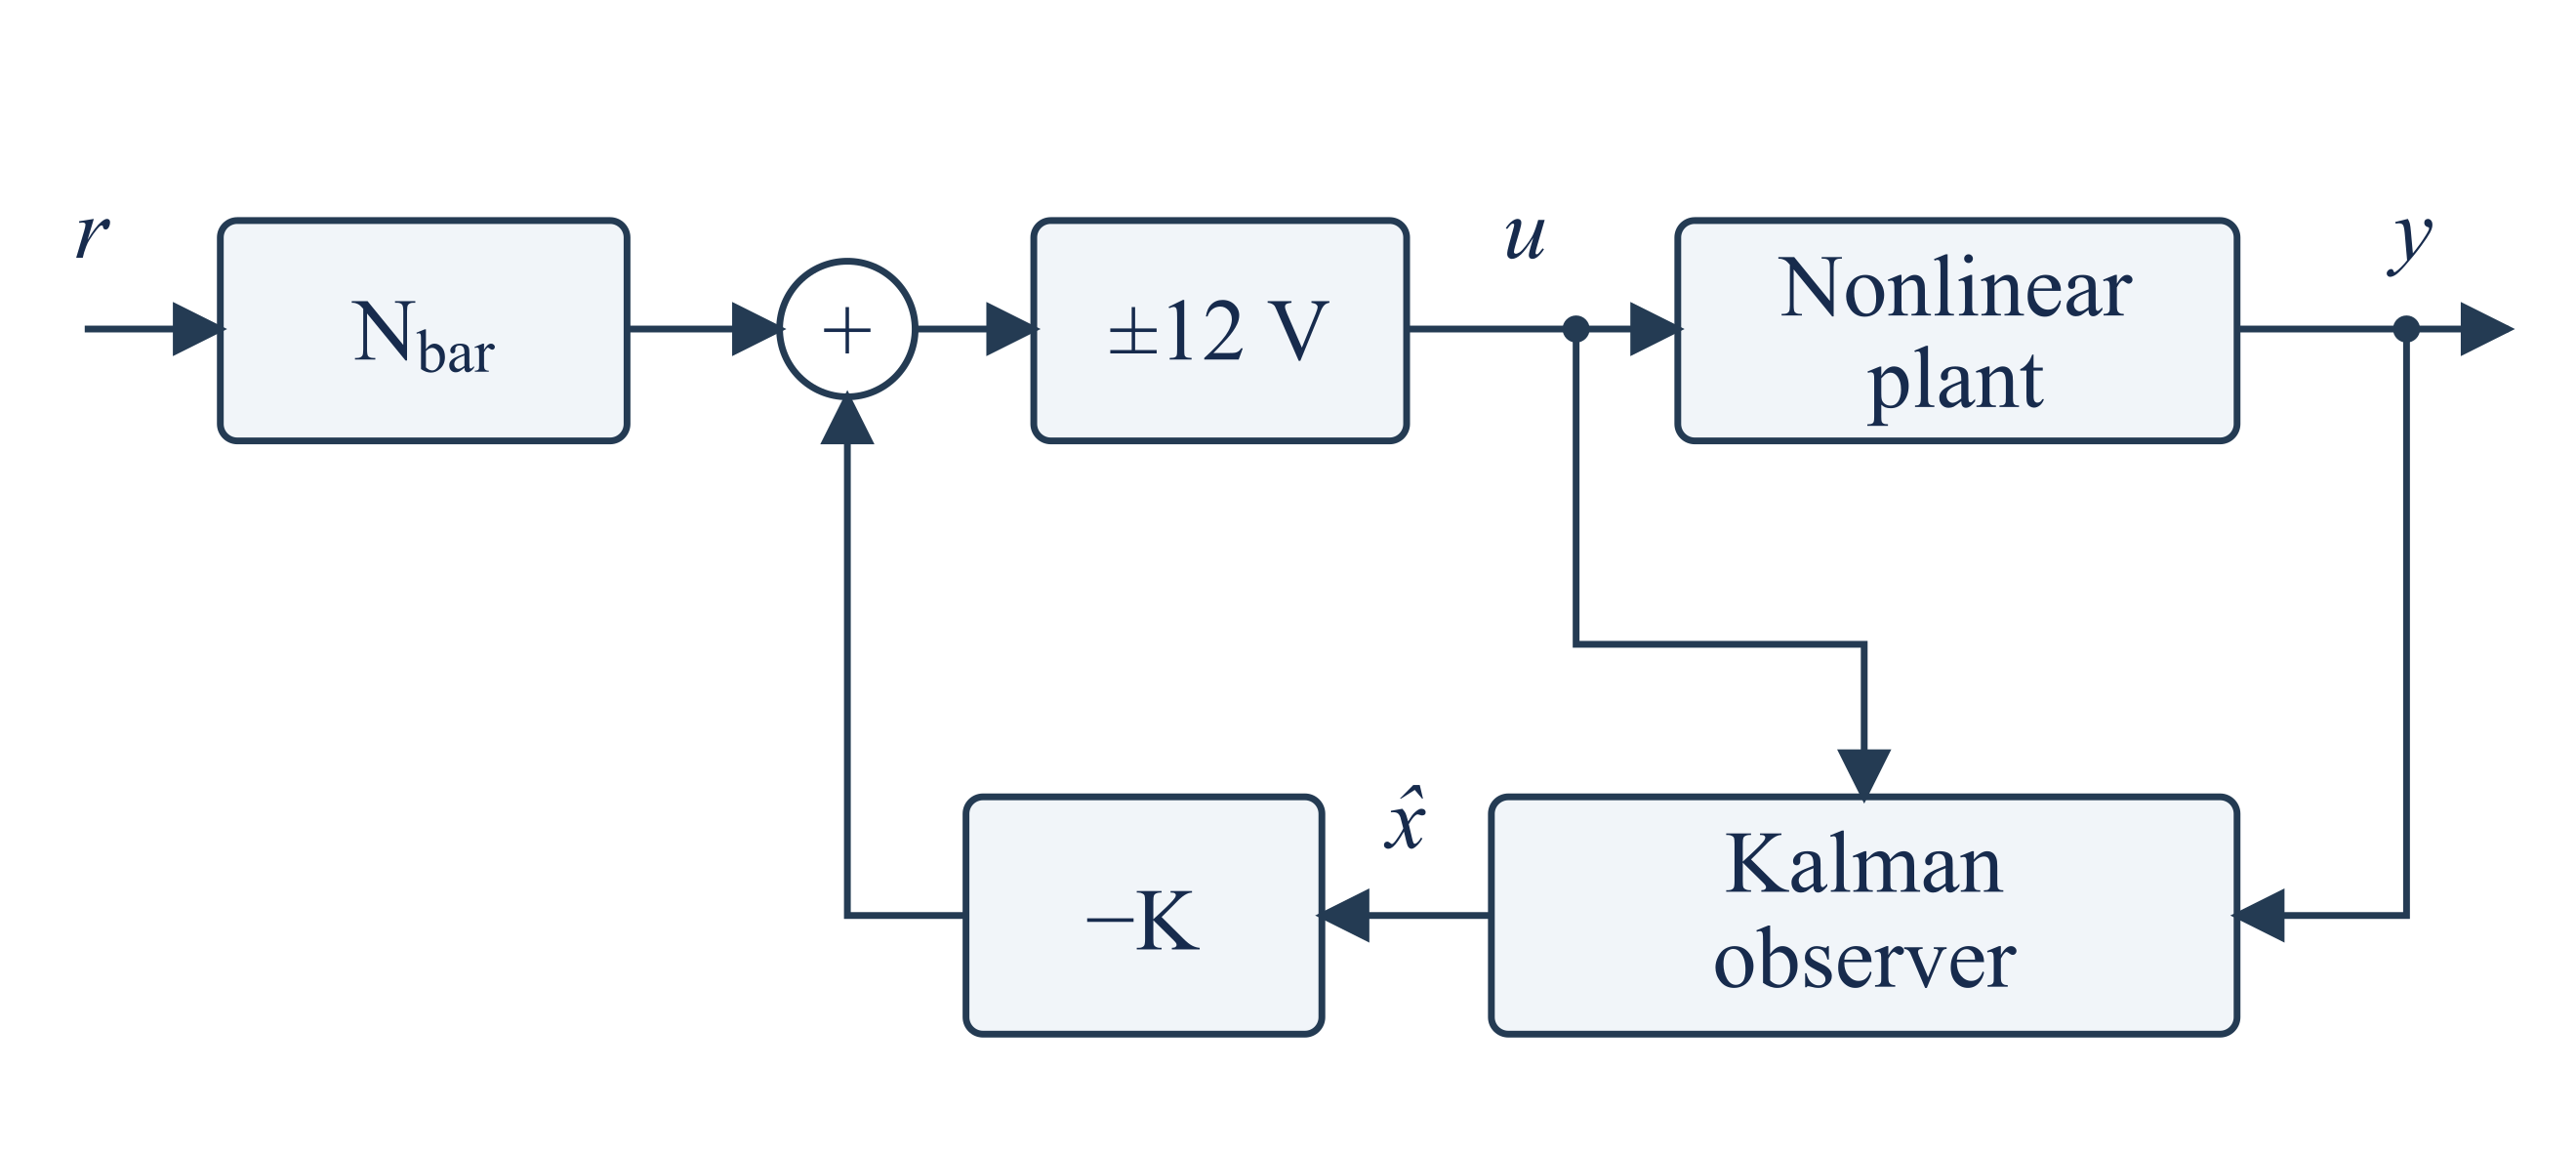
\includegraphics[width=\columnwidth]{control_structure.png}
\caption{Reference feedforward with LQR feedback and Kalman state estimation.}
\label{fig:structure}
\end{figure}

\subsection{Reference Tracking Results}

The controller is evaluated in a $40$ s nonlinear Simulink simulation with $\alpha(0)=5^\circ$, all other physical states initially zero, and $\hat x(0)=0$. The first $8$ s allow the pendulum to recover before the arm reference changes according to

\begin{equation}
r(t)=\begin{cases}
0^\circ,&0\le t<8,\\
20^\circ,&8\le t<16,\\
-15^\circ,&16\le t<24,\\
30^\circ,&24\le t<32,\\
0^\circ,&32\le t\le40.
\end{cases}
\label{eq:reference}
\end{equation}

Tracking accuracy is measured using $e=r-\theta$. For each constant-reference interval, the maximum absolute error during its final second is

\begin{equation}
E_{\mathrm{tail}}=\max_{t_k\in[t_f-1,t_f]}|e(t_k)|,
\label{eq:tailmetric}
\end{equation}

where $t_f$ is the final sample time of that interval. Figure \ref{fig:tracking} and Table \ref{tab:tracking} present the simulated response and tracking performance.

\begin{figure}[t]
\centering
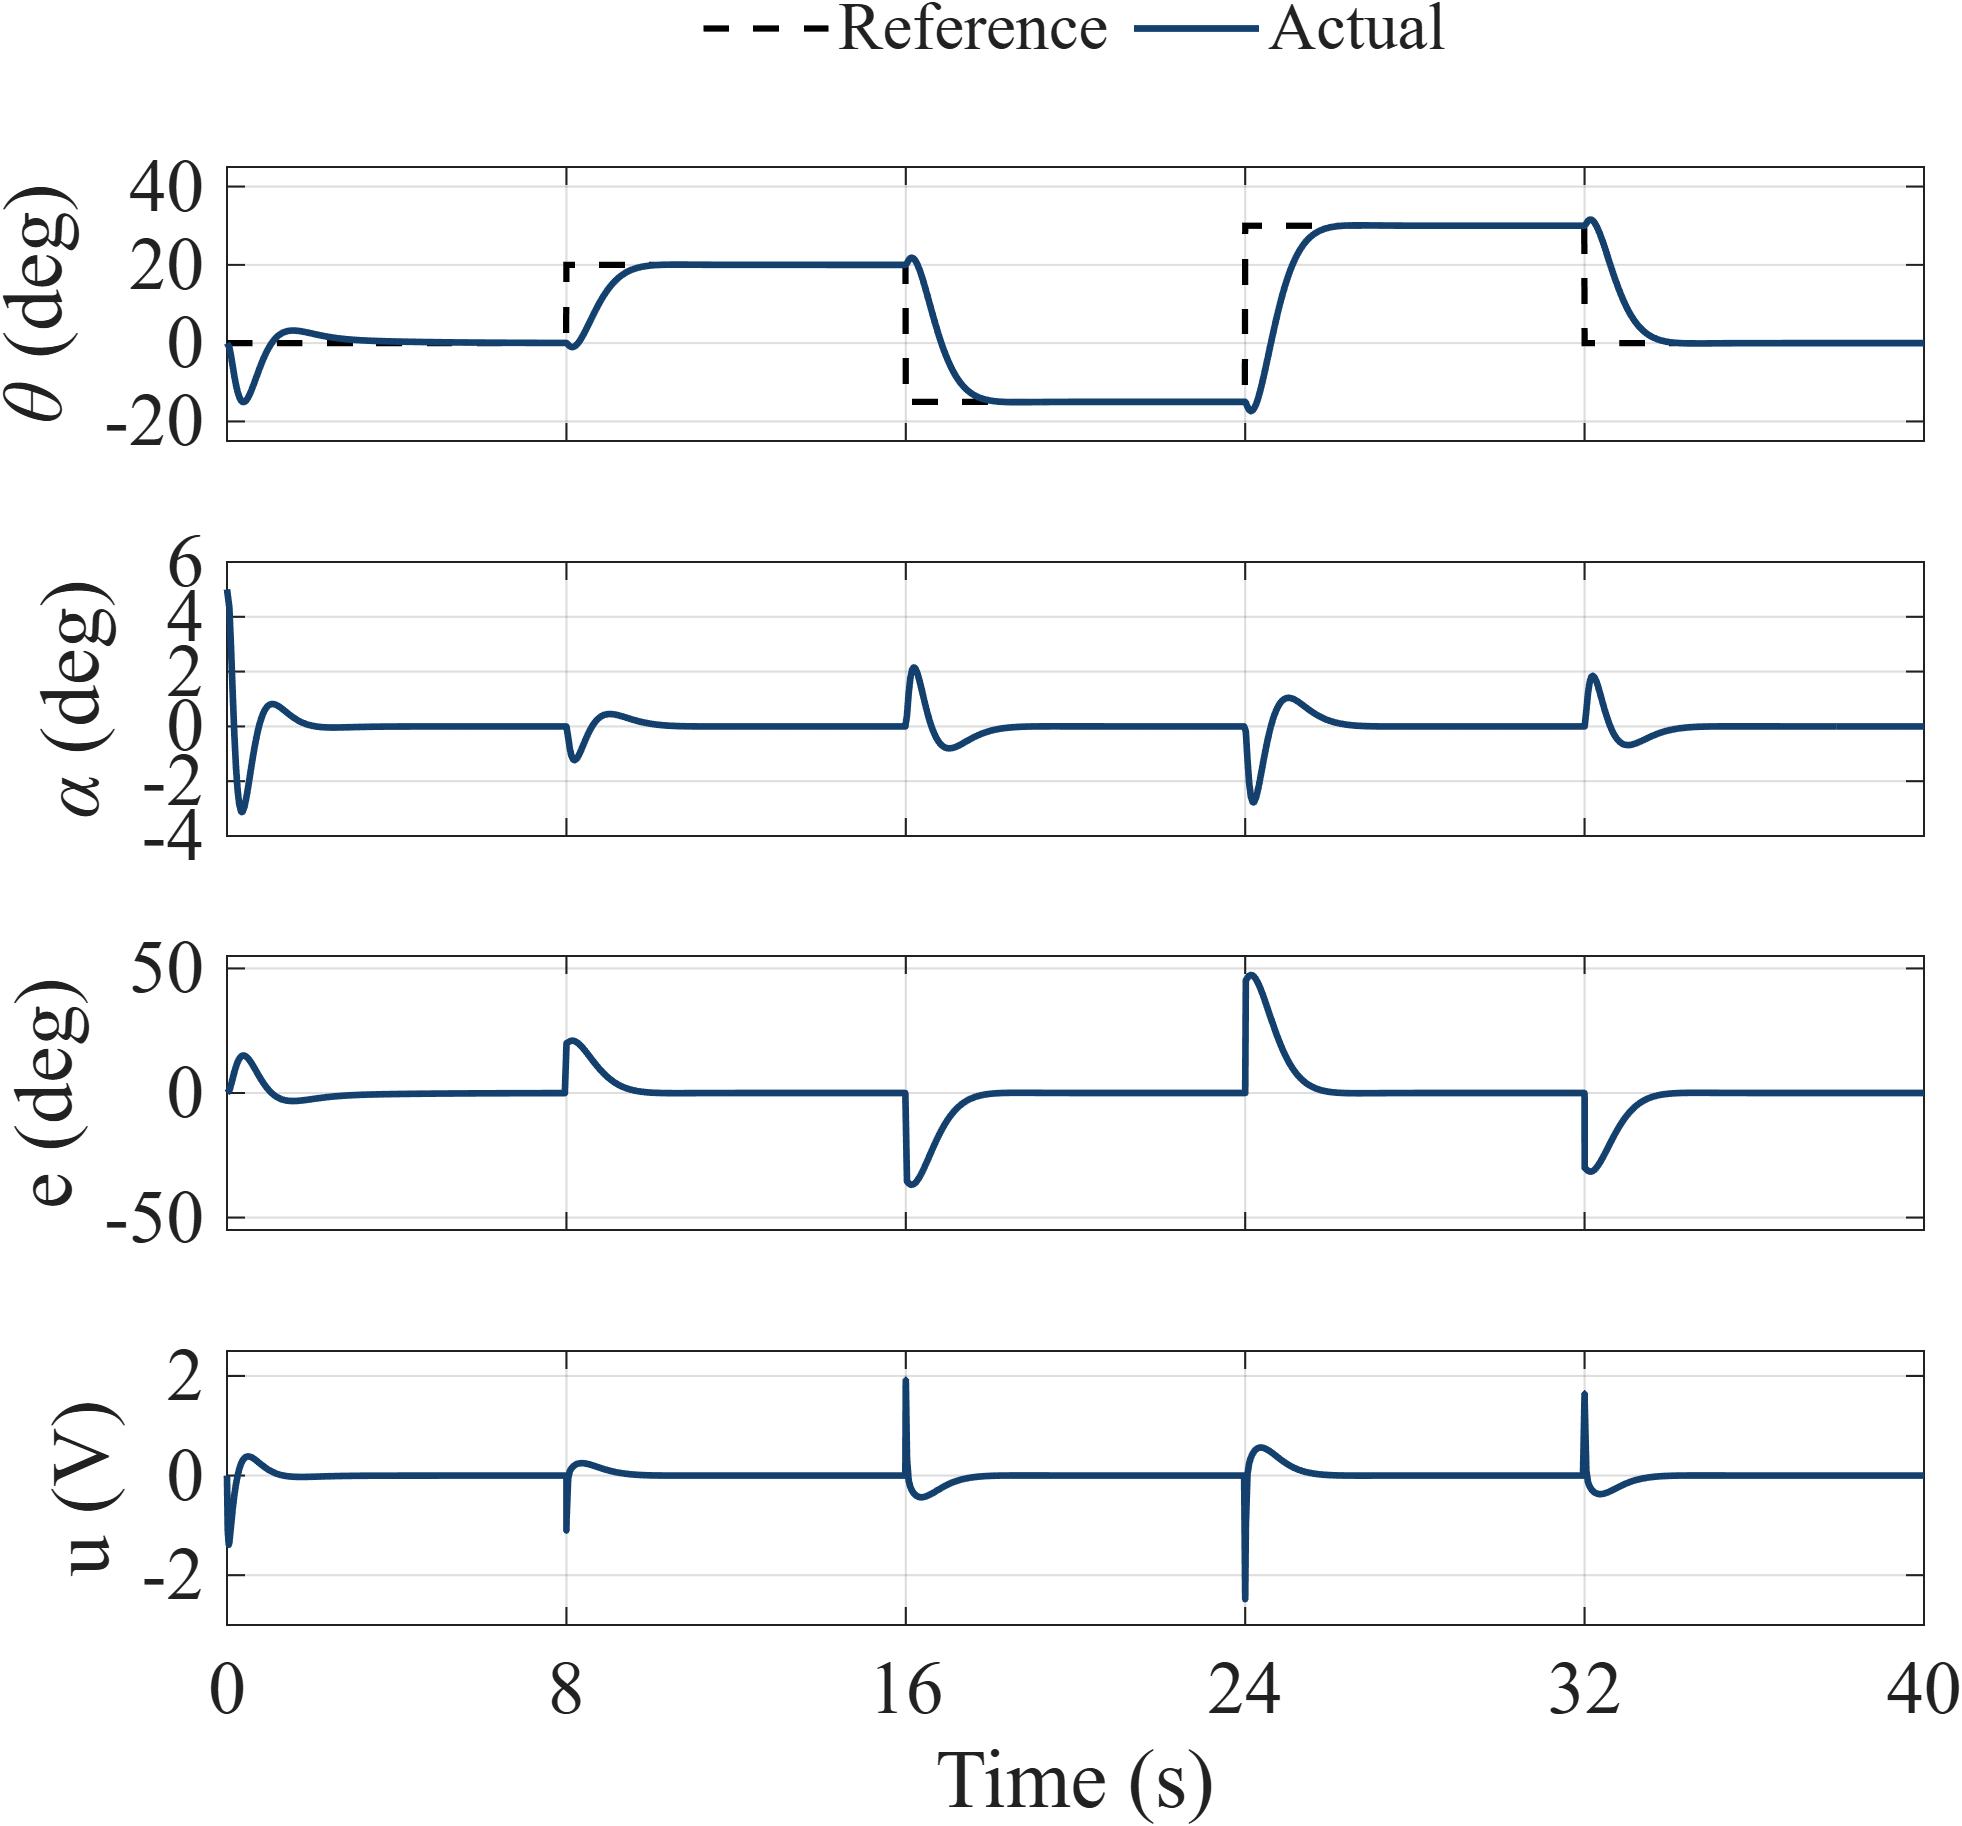
\includegraphics[width=\columnwidth]{step3_tracking.png}
\caption{Nonlinear feedforward tracking of $0^\circ$, $20^\circ$, $-15^\circ$, $30^\circ$, and $0^\circ$.}
\label{fig:tracking}
\end{figure}

\begin{table}[t]
\caption{Feedforward Tracking Performance}
\label{tab:tracking}
\centering\small
\begin{tabular}{@{}ccccc@{}}
\toprule
Start & Target & Peak $|\alpha|$ & $E_{\mathrm{tail}}$ & Peak $|u|$\\
(s) & ($^\circ$) & ($^\circ$) & ($^\circ$) & (V)\\
\midrule
8 & $20$ & 1.2321 & $7.9629\!\times\!10^{-4}$ & 1.1041\\
16 & $-15$ & 2.1569 & $1.2119\!\times\!10^{-4}$ & 1.9317\\
24 & $30$ & 2.7747 & $2.7664\!\times\!10^{-4}$ & 2.4836\\
32 & $0$ & 1.8483 & $7.8304\!\times\!10^{-5}$ & 1.6558\\
\bottomrule
\end{tabular}
\end{table}

The arm reaches each commanded angle while the pendulum returns upright after each switch. The largest reference change, from $-15^\circ$ to $30^\circ$, produces the largest post-switch pendulum deviation, $2.7747^\circ$, and the highest voltage peak, $2.4836$ V. Across the four switched intervals, the maximum final-second arm error is $0.000796291^\circ$, and the maximum pendulum deviation over those windows is $5.2881\!\times\!10^{-6}\,^\circ$.

The initial $0$--$8$ s recovery interval has a final-second arm error of $0.0746441^\circ$. Reference changes produce an immediate feedforward voltage adjustment followed by state-feedback correction. The full-run peak voltage is $2.4836$ V, below the $12$ V limit, so the limiter remains inactive throughout this test.

\section{Conclusion}

The Kalman observer estimates the unmeasured angular velocities from the two measured angles, allowing the selected LQR controller to recover the pendulum from an initial $5^\circ$ tilt. A reference feedforward gain extends the same feedback design to arm-angle tracking. The nonlinear simulation follows four reference changes with a maximum final-second tracking error of $0.000796291^\circ$ and a peak motor voltage of $2.4836$ V. The pendulum returns upright after each change, consistent with the closed-loop stability and nominal steady-state tracking analysis.


\clearpage
\appendices

\noindent\begin{minipage}{\columnwidth}
\section{step1.m}
\begin{lstlisting}
function [plant, observer] = step1
% Preserve the supplied upright linearization and four-state LQE design.
plant_parameters;
plant = struct('mp',mp,'r',r,'Lp',Lp,'lp',lp,'J',J,'Jp',Jp, ...
    'eta_g',eta_g,'G',G,'eta_m',eta_m,'kt',kt,'Ra',Ra,'kb',kb, ...
    'Bp',Bp,'Br',Br,'g',g);
Marm = J + mp*r^2;
Hpend = Jp + mp*lp^2;
couple = mp*lp*r;
hgrav = mp*lp*g;
kVoltage = eta_g*G*eta_m*kt/Ra;
dampingVoltage = Br + kVoltage*G*kb;
Delta = Marm*Hpend - couple^2;
assert(Delta > 0, 'Linearized mass matrix is singular/nonphysical.');

A = [0, 0,                     1,                       0;
     0, 0,                     0,                       1;
     0, couple*hgrav/Delta,   -Hpend*dampingVoltage/Delta, -couple*Bp/Delta;
     0, Marm*hgrav/Delta,     -couple*dampingVoltage/Delta, -Marm*Bp/Delta];
B = [0; 0; Hpend*kVoltage/Delta; couple*kVoltage/Delta];
C = [1 0 0 0; 0 1 0 0];
D = zeros(2,1);
Gnoise = [zeros(2); eye(2)];
Qn = 10*eye(2);
Rn = eye(2);
L = lqe(A,Gnoise,C,Qn,Rn);
A_obs = A-L*C;
B_obs = [B L];
C_obs = eye(4);
D_obs = zeros(4,3);
assert(rank(ctrb(A,B))==4 && rank(obsv(A,C))==4);
assert(all(real(eig(A_obs))<0));
observer = struct('A',A,'B',B,'C',C,'D',D,'Gnoise',Gnoise, ...
    'Qn',Qn,'Rn',Rn,'L',L,'A_obs',A_obs,'B_obs',B_obs,'C_obs',C_obs,'D_obs',D_obs);
fprintf('STEP1_OK | controllability 4/4 | observability 4/4\n');
disp('LQE gain L ='); disp(L);
end
\end{lstlisting}
\end{minipage}
\par\medskip

\noindent\begin{minipage}{\columnwidth}
\section{lqr\_design.m}
\begin{lstlisting}
function design = lqr_design(observer)
% LQR design function for nonlinear simulations; uses the same cases as step2.m.
if nargin==0
    [~,observer] = step1;
end
A = observer.A;
B = observer.B;
Q_values = [10 100 1 10; 10 300 1 10; 10 100 1 10; 10 100 1 10];
R_values = [1 1 0.1 10];
t = (0:0.01:5)';
x0 = [0; deg2rad(5); 0; 0];
K_all = zeros(4,4);
angles = zeros(numel(t),4);
pendulum = angles;
voltage = angles;
for index = 1:4
    K = lqr(A,B,diag(Q_values(index,:)),R_values(index));
    K_all(index,:) = K;
    closedLoop = ss(A-B*K,zeros(4,1),eye(4),zeros(4,1));
    x = initial(closedLoop,x0,t);
    angles(:,index) = rad2deg(x(:,1));
    pendulum(:,index) = rad2deg(x(:,2));
    voltage(:,index) = -x*K';
end
selected_case = 2;
K = K_all(selected_case,:);
Q = diag(Q_values(selected_case,:));
R = R_values(selected_case);
assert(all(real(eig(A-B*K))<0));
caseNumber = (1:4)';
comparison = table(caseNumber,Q_values(:,2),R_values',max(abs(angles))', ...
    max(abs(voltage))',caseNumber==selected_case, ...
    'VariableNames',{'Case','Q_alpha','R','PeakArm_deg','PeakVoltage_V','Selected'});
design = struct('Q',Q,'R',R,'K',K,'comparison',comparison,'t',t, ...
    'angles',angles,'pendulum',pendulum,'voltage',voltage);
disp(comparison);
fprintf('STEP2_OK | selected case %d\n',selected_case);
end
\end{lstlisting}
\end{minipage}
\par\medskip

\noindent\begin{minipage}{\columnwidth}
\section{step3.m}
\begin{lstlisting}
function design = step3(observer, baseline)
% Reference feedforward using the LQR gain selected in Step 2.
if nargin<1, [~,observer] = step1; end
if nargin<2, baseline = lqr_design(observer); end
A = observer.A;
B = observer.B;
Ctheta = observer.C(1,:);
K = baseline.K;
steady = [A B; Ctheta 0] \ [zeros(4,1); 1];
Nx = steady(1:4);
Nu = steady(5);
Nbar = Nu + K*Nx;
poles = eig(A-B*K);
dcGain = -Ctheta*((A-B*K)\(B*Nbar));
assert(all(real(poles)<0), 'Reference-tracking regulator is unstable.');
assert(abs(dcGain-1)<1e-10, 'Reference prefilter must give unit DC gain.');
design = struct('Q',baseline.Q,'R',baseline.R,'Kx',K, ...
    'Nx',Nx,'Nu',Nu,'Nbar',Nbar,'poles',poles,'dcGain',dcGain, ...
    'voltageLimit',12);
fprintf('STEP3_DESIGN_OK | K = %s | Nbar = %.8f | DC gain = %.12f\n', ...
    mat2str(K,8),Nbar,dcGain);
end
\end{lstlisting}
\end{minipage}
\par\medskip

\end{document}
